\section{问题四的模型建立与求解}

\subsection{求解思路与模型选择}

问题四是在问题二、三的基础上进一步考虑外网电价的实时波动。前文已经解决了负载与光伏预测、误差准备、储能调度和订单调整问题，本问真正新增的困难是：制定订单时，未来各时段的实际电价也尚未发生。如果仍按固定电价安排储能，就可能在并不便宜的时段提前充电，或在后面更高的价格到来之前过早放空电池。因此，波动电价不仅改变最终账单，也会改变购电和充放电时点。

本问仍分为两种运行方式。对应问题二时，每天只能在0:00确定当天订单，之后即使电价判断发生偏差也不能改单；对应问题三时，6:00、12:00和18:00可以根据已经发生的价格、最新光伏预报和实际库存重新安排未执行订单。两种运行方式的信息条件不同，价格模型也不宜简单照搬。

为此，我们设置三个价格候选。历史同刻中位数直接保留稳定的日内峰谷和星期规律，可作为容易解释的基准；岭回归能够利用多项相关历史信息，并用正则项限制系数过度波动；直方图梯度提升树则擅长表达价格、净负荷、星期和季节之间的非线性组合。三种方法使用相同的历史信息、供需预测、初始储电量和结算规则，最终按照实际购电费用、紧急购电量和可解释性共同选择。价格预测完成后，将预测价格代入前文的线性规划；供需平衡、储能递推、容量与功率限制均沿用问题二、三，不再重复建立。

从题意看，只在零点制定计划时，没有当天已发生价格可用，历史因素之间的非线性组合更重要，因此预先把提升树作为问题四-2的重点方案；允许日内调整时，模型需要频繁根据新信息解释价格修正，稳定而透明的岭回归更符合问题四-3的运行方式。后续实际比较表明，前一判断得到最低费用支持；后一分支中，岭回归虽然比提升树多花2273.23元，但紧急购电减少1382.32~kWh，且各项修正的含义更清楚。因此，两条分支分别采用：

\textbf{问题四-2：滚动提升树--零点线性规划模型。}

\textbf{问题四-3：滚动岭回归--日内调整线性规划模型。}

\subsection{波动电价的规律与预测依据}

前文已经说明，同一日内时刻的电价在不同日期之间仍有明显波动。本问进一步围绕“哪些历史信息能够在决策时使用”作定量比较，得到三个直接结论：\textbf{电价具有稳定的日内峰谷轮廓；上周同刻比前一天同刻更有参考价值；日内已经发生的价格可以修正当天后续判断。}

首先，全年同刻均价在05:40附近最低，约为0.3713元/kWh，在20:40附近最高，约为1.3952元/kWh；83.29\%的日最高价落在19:00--22:00。每天价格曲线与全年同刻均值曲线的平均相关系数达到0.9706，说明“夜间较低、晚间较高”的基本形状较稳定。不过，同一时刻的实际价格仍有明显变化，所以固定日曲线只能提供骨架，不能直接替代每天的价格判断。

其次，以已经发生的数据作参照时，上周同刻价格的平均绝对误差约为0.0466元/kWh，前一天同刻约为0.0845元/kWh。这与前文发现的周规律相符，因此模型同时使用过去四周相同星期位置的中位数、最近七天同刻中位数和上周同刻价格。中位数不容易被个别异常高价带偏，更适合作为滚动预测的历史基线。

最后，扣除同刻平均轮廓后，实际净负荷与价格偏差的相关系数约为0.9165。由此在特征中加入决策时点能够得到的预测净负荷，但不使用未来真实负载和光伏，也不把这种统计关系解释为因果。日内分支还利用当天已经发生的价格：若0:00至当前时刻的价格整体高于历史基线，则适当上调后续判断；最近一个区间的偏差则用于描述短时变化。对于尚未发生的价格，模型始终只使用决策时点之前的信息。

\subsection{数学模型的建立}

记$d$为日期，$k=1,2,\ldots,144$为当天的十分钟时段，$r$为当前决策时点。$p_{d,k}$和$\widehat p_{d,k|r}$分别表示实际电价和在$r$时刻作出的预测。价格特征向量记为$\boldsymbol x_{d,k|r}$，它由历史同刻价格、预测净负荷、星期位置、年内位置、预测提前量等组成；在6:00、12:00和18:00，还加入当天已经发生价格相对历史基线的偏差。

两个价格模型均每7天更新一次，只使用最近56天内已经兑现的历史样本。历史不足56天时使用当时已有的数据。构造训练样本时按历史决策时点还原可用信息，尚未发生的目标价格不进入训练。每天四次更新的是输入和预测结果，并非一天重新训练四次模型。

\subsubsection{问题四-2：滚动提升树--零点线性规划模型}

零点还没有当天已经发生的价格可供修正，价格判断主要依靠周周期、近期价格、季节位置和预测净负荷。线性模型难以充分表达这些因素在不同价格区间下的组合关系，因此采用直方图梯度提升树。模型从一个初始价格判断开始，每棵树继续修正上一轮没有拟合好的部分：
\begin{equation}
 F_M(\boldsymbol x)=F_0(\boldsymbol x)+\gamma\sum_{m=1}^{M}h_m(\boldsymbol x),
 \qquad \widehat p_{d,k|0}=\max\{0.001,F_M(\boldsymbol x_{d,k|0})\}.
 \label{eq:q42tree}
\end{equation}
其中，$h_m$为第$m$棵回归树，$M=100$，学习率$\gamma=0.05$。最终每棵树最多31个叶节点，每个叶节点至少包含50个训练样本。31个叶节点表示一棵树最多区分31种特征组合，不是31棵树，也不是一天作31次购电决定。

得到预测价格后，沿用问题二的预测净需求$n_t$、普通订单$q_t$、外网充电$x_t$、电池放电$z_t$和储电量$S_t$。问题二的近期误差准备、储能递推和容量功率限制保持不变，只将固定电价换为当前预测的波动电价，求解
\begin{equation}
 \min\ J_{4-2}=\sum_{t\in\mathcal T_0}\widehat p_{t|0}q_t-\nu S_T,
 \qquad q_t=n_t-z_t+x_t.
 \label{eq:q42lp}
\end{equation}
规划窗口延伸到次日24:00，以避免模型在当天末尾无意义地放空电池，但只固定当天144个时段的普通订单。$\nu S_T$表示规划末端剩余电量的参考价值，仅用于安排库存，不作为售电收入从实际费用中扣除。白天按附件2的实际供需运行，普通订单不足时先由电池补充，仍不足的部分再按实际电价的5倍紧急购电。

\subsubsection{问题四-3：滚动岭回归--日内调整线性规划模型}

日内分支在6:00、12:00和18:00可以看到当天已经发生的价格。上周同刻、四周同星期中位数、最近七天中位数以及当天价格偏差之间具有较强相关性。普通线性回归可能给相近特征分配很大的正负系数，再依靠彼此抵消降低训练误差，导致预测对小幅变化过于敏感。为限制这种不稳定，采用岭回归。

先按当前训练集的均值和标准差将各特征标准化为$z_{ij}$，然后求解
\begin{equation}
 \min_{\beta_0,\boldsymbol\beta}
 \sum_{i\in\mathcal I_r}\left(p_i-\beta_0-\sum_j\beta_jz_{ij}\right)^2
 +\lambda\sum_j\beta_j^2,
 \qquad \lambda=10,
 \label{eq:ridge}
\end{equation}
并令
\begin{equation}
 \widehat p_{d,k|r}=\max\left\{0.001,\beta_0+
 \boldsymbol z_{d,k|r}^{\mathsf T}\boldsymbol\beta\right\}.
 \label{eq:ridgepredict}
\end{equation}
式\eqref{eq:ridge}第一项要求预测接近已发生价格，第二项压缩过大的系数，截距不受惩罚。这里的系数由历史数据拟合，可以为负，也不要求和为1；它们不是人为分配的权重。$\lambda=10$是候选阶段采用的固定设置，后面的残差模型检验不作为该参数的选取依据。

日内每次更新预测价格后，沿用问题三的光伏预报融合、误差准备、储能约束和改单结算。设$q_t^0$为零点原计划，$q_t$为当前调整后的订单，$e_t$为预计紧急购电量。用辅助变量$\delta_t$表示订单相对零点计划的净变化：
\begin{equation}
 \delta_t\ge q_t-q_t^0,\qquad \delta_t\ge q_t^0-q_t,
 \qquad t\in\mathcal D_r,
 \label{eq:delta}
\end{equation}
其中，$\mathcal D_r$为当天尚未执行的时段。滚动优化目标为
\begin{equation}
 \min\ J_{4-3}=\sum_{t\in\mathcal T_r}\widehat p_{t|r}(q_t+5e_t)
 +\frac12\sum_{t\in\mathcal D_r}\widehat p_{t|r}\delta_t-\nu S_T.
 \label{eq:q43lp}
\end{equation}
由于调整费用为正，最优解中$\delta_t=|q_t-q_t^0|$。已执行区间保持不变，多次调整同一时段时，只按最终订单相对零点计划的净变化结算，避免重复收费。规划使用预测价格，最终普通购电、调整和紧急购电均按该时段实际价格结算。

\subsection{模型求解与结果分析}

两条分支在价格给定后均为线性规划，采用HiGHS求解。2025年1月从题给6000~kWh电量连续运行，用于形成历史和确定2月初实际库存；正式统计2025年2月1日至12月31日，共334天。为公平比较价格方法，六套候选统一从2月1日8592.69~kWh开始，供需预测、设备条件和费用口径完全相同。

\subsubsection{候选比较与模型确定}

三种价格方法接入相同调度模型后的结果见表\ref{tab:q4compare}。预测误差采用全部时段的平均绝对误差，总费用按实际电价和真实供需重新结算。

\begin{table}[htbp]
\centering\small
\caption{波动电价下三种价格方法的比较}
\label{tab:q4compare}
\begin{tabular}{llrrr}
\toprule
对应分支 & 价格方法 & 价格MAE/(元/kWh) & 总费用/万元 & 紧急购电量/kWh \\
\midrule
问题四-2 & 历史同刻中位数 & 0.04984 & 1427.22 & 97728.89 \\
问题四-2 & 岭回归 & 0.04472 & 1426.64 & 99205.19 \\
问题四-2 & 提升树 & 0.03884 & 1425.52 & 98725.98 \\
问题四-3 & 历史同刻中位数 & 0.04676 & 1383.78 & 40144.52 \\
问题四-3 & 岭回归 & 0.04442 & 1382.29 & 38733.80 \\
问题四-3 & 提升树 & 0.03834 & 1382.06 & 40116.12 \\
\bottomrule
\end{tabular}
\end{table}

虽然建模前已经根据零点信息条件优先考虑提升树，我们仍将三个候选接入同一调度模型实跑。问题四-2中，提升树比岭回归少花11190.77元，并取得最低的价格预测误差，说明非线性组合确实有助于零点判断。随后将每棵树的最大叶节点数由15增加到31，总费用进一步减少6605.53元，最终采用31叶版本。

问题四-3中，提升树的总费用比岭回归低2273.23元，仅占岭回归总费用的0.016\%；但其紧急购电量多1382.32~kWh，发生紧急购电的日期也多2天。逐日比较中，提升树有165天更便宜、169天更贵，优势并不稳定。日内策略需要反复更新，岭回归能够直接说明历史价格、当前偏差和净负荷怎样共同修正后续价格，且对高度相关的输入更稳定。因此，我们保留结构清楚、紧急购电较少的岭回归方案，并将这2273.23元视为降低运行风险和提高可解释性所付出的代价。这里的选择说明模型比较并非只取费用表中最小的一行，还要看风险和实际使用方式是否匹配。

\subsubsection{最终费用与指定日期结果}

两条最终策略的全年费用见表\ref{tab:q4result}。允许日内调整的方案虽然增加了调整费，但普通购电费和紧急购电费更低，最终比零点一次订电少花425669.52元，约2.99\%。这一差额同时包含日内供需信息、价格更新、误差准备和改单权限的作用，不能全部解释为价格更新的收益。

\begin{table}[htbp]
\centering\small
\caption{问题四两条分支的全年费用结果}
\label{tab:q4result}
\begin{tabular}{lrr}
\toprule
指标 & 问题四-2 & 问题四-3 \\
\midrule
普通购电费/元 & 13613522.32 & 13327163.05 \\
调整费/元 & 0.00 & 268515.82 \\
紧急购电费/元 & 635048.55 & 227222.48 \\
总费用/元 & 14248570.87 & 13822901.35 \\
紧急购电量/kWh & 98756.33 & 38733.80 \\
期末储电量/kWh & 8692.34 & 7918.81 \\
\bottomrule
\end{tabular}
\end{table}

题目指定日期的主要运行结果见表\ref{tab:q4days}。同一天中，两条策略可能得到不同的日末库存和费用，说明波动价格下的调度差异会沿储电状态传递到下一天。普通订单表示需要付费的最终订单量，不等于全部被负载或电池实际接收的电量。

\begin{table}[htbp]
\centering\footnotesize
\caption{问题四指定日期的购电与储电结果}
\label{tab:q4days}
\begin{tabular}{llrrrr}
\toprule
分支 & 日期 & 最终普通订单/kWh & 紧急购电/kWh & 日末储电/kWh & 总费用/元 \\
\midrule
问题四-2 & 3月20日 & 62329.63 & 329.13 & 1376.30 & 41909.16 \\
问题四-2 & 6月21日 & 42375.21 & 0.00 & 10380.22 & 20358.11 \\
问题四-2 & 9月23日 & 68066.93 & 10.23 & 2592.35 & 44700.97 \\
问题四-2 & 12月21日 & 94612.77 & 0.00 & 9798.14 & 71357.71 \\
问题四-3 & 3月20日 & 61795.52 & 93.27 & 1311.14 & 40921.66 \\
问题四-3 & 6月21日 & 42176.92 & 14.64 & 10800.00 & 20204.97 \\
问题四-3 & 9月23日 & 67751.81 & 11.32 & 3463.77 & 45250.33 \\
问题四-3 & 12月21日 & 93283.52 & 20.53 & 8131.62 & 71876.82 \\
\bottomrule
\end{tabular}
\end{table}

\subsection{模型检验与结论}

我们主要检查了三件事。第一，重新读取保存的订单和储电轨迹，逐段核对供需平衡、容量、充放电功率、信息截止时点和实际费用。共核对865728个十分钟运行区间，储电递推最大误差约为$9.09\times10^{-13}$~kWh，全年总账最大差约为$1.86\times10^{-9}$元，均属于数值计算误差。

第二，检验模型选择是否过分依赖单一设置。图\ref{fig:q4check}(a)表明，在7、15和31叶三个设置中，31叶树的全年费用最低；但它仍有149天和4个月比15叶树更贵，因此只能说在本年所比较的设置中表现较好。对于日内岭回归，我们尝试了先确定历史基线、再预测价格偏差的残差模型，三组正则强度均未降低费用，故仍保留完整岭回归。

第三，单独考察当天已发生价格的作用。保持光伏预报、实际库存和改单权限不变，全天沿用零点价格判断会多花274.45元；分别不使用6:00、12:00和18:00价格更新，费用变化为$+59.37$元、$-27.40$元和$+312.58$元，如图\ref{fig:q4check}(b)所示。12:00更新没有带来节费，说明新信息并不保证每次调整都更划算；各次更新会共同改变后续库存，费用差不能直接相加。

\begin{figure}[htbp]
\centering
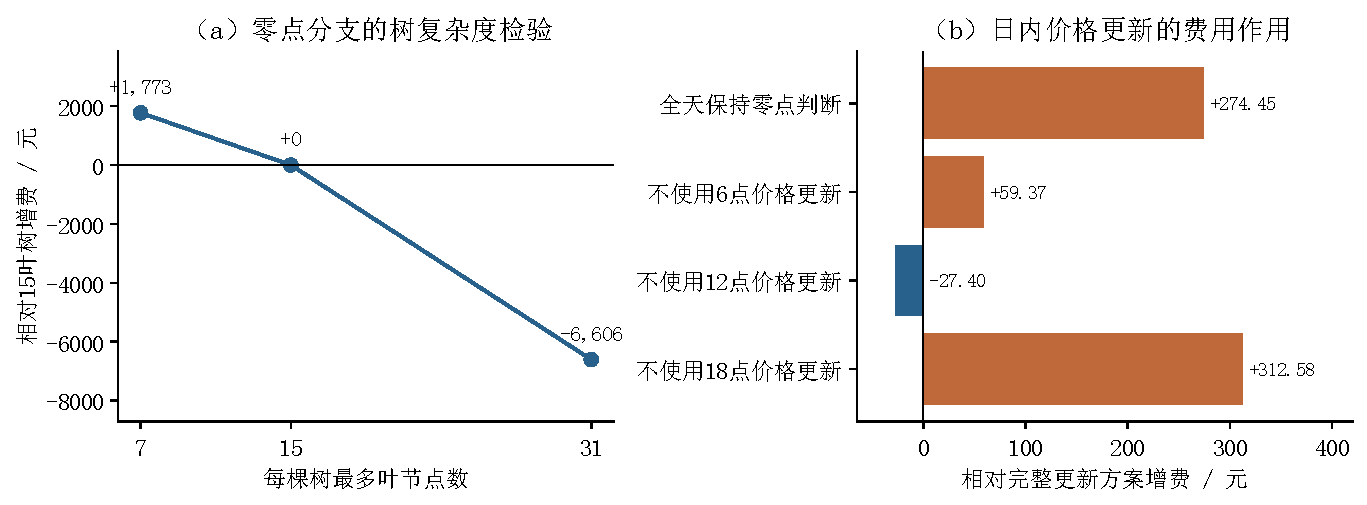
\includegraphics[width=.96\linewidth]{问题四模型检验.pdf}
\caption{树复杂度与日内价格更新的费用检验}
\label{fig:q4check}
\end{figure}

在实际价格最高的5\%区间内，问题四-2仍有46086.96~kWh紧急购电，问题四-3仍有14665.07~kWh。这说明储能受容量和放电功率限制，不能完全消除连续高价与供需偏差叠加的风险。进一步对期末库存按三档价格估值后，31叶树相对15叶树仍节省5890.24--6423.72元，说明它并非仅靠少留库存降低费用。

综上，波动电价下应先利用历史价格和当前可得信息判断未来价格，再通过线性规划统一安排普通购电与储能。问题四-2采用滚动提升树--零点线性规划模型，总费用为14248570.87元；问题四-3采用滚动岭回归--日内调整线性规划模型，总费用为13822901.35元。现有检验支持这两种模型在2025年数据范围内的选择，但参数比较仍基于同一年数据，结论不能直接推广到其他年份或其他微网。
